\section{Resting atmosphere}
\label{sec:resting}

This two-dimensional test simulates a stably stratified atmosphere in hydrostatic balance.  Since there are no net forces, the analytic solution should remain at rest.  The test specification follows that from \textcite{klemp2011}, and challenges the accuracy of the calculation of the horizontal pressure gradient.  An inversion layer causes nonlinear processes that further tax the model \autocite{good2013}.

\subsection{Specification}
Following \textcite{weller-shahrokhi2014}, the domain is \SI{20}{\kilo\meter} wide and \SI{20}{\kilo\meter} high, which is narrower than \textcite{klemp2011} in order to reduce simulation time.  The wave-shaped mountain profile is taken from \textcite{schaer2002} where the surface height $h$ is given by
\begin{align}
	\surface(x) = \surface_0 \exp \left( - \left( \frac{x}{a} \right)^2 \right) \cos^2 \left( \frac{\pi x}{\lambda} \right) \label{eqn:resting:mountain}
\end{align}
where $a = \SI{5}{\kilo\meter}$ is the mountain half-width, $h_0 = \SI{1}{\kilo\meter}$ is the maximum mountain height and $\lambda = \SI{4}{\kilo\meter}$ is the wavelength.  For the optimised SLEVE grid, the large-scale component $\surface_1$, described in section~\ref{sec:theory:tf}, is specified as
\begin{align}
\surface_1(x) = \frac{1}{2} \surface_0 \exp \left( - \left( \frac{x}{a} \right)^2 \right)
\end{align}
and, following \cite{leuenberger2010}, $s_1 = \SI{4}{\kilo\meter}$ is the large scale height, $s_2 = \SI{1}{\kilo\meter}$ is the small scale height, and the optimal exponent value of $n = 1.35$ is used.  Results are compared with the numerical solution with no orography.

The initial thermodynamic conditions have a surface temperature of $\theta_0 = \SI{288}{\kelvin}$ and constant stability with Brunt-V\"ais\"al\"a frequency $N = \SI{0.01}{\per\second}$ everywhere, except for a more stable layer of $N = \SI{0.02}{\per\second}$ between $\SI{2}{\kilo\meter} \leq z \leq \SI{3}{\kilo\meter}$.

\subsection{Diagnostics}
Two metrics were used to measure the model error.  First, maximum vertical velocity is measured at each timestep.  An analytic solution has no vertical velocity $w$ since the atmosphere is at rest.  However, numerical error in calculating the horizontal pressure gradient give rise to spurious vertical velocities which become more severe over steep terrain \autocite{klemp2011}.

Second, normalised energy change $\Delta E$ is measured for each timestep as described in section~\ref{sec:method:energy}.  The total normalised energy change is the sum of normalised kinetic, potential, and internal energy changes.
An analytic solution would conserve total energy such that $\Delta E(t) = 0\;\forall\;t$.  As discussed in \textcite{weller-shahrokhi2014}, energy is not exactly conserved in the model presented because of damping by the advection scheme and inexact transfer between kinetic, internal and potential energy.

\subsection{Discretisation}
The simulation uses the discretisation of the fully-compressible Euler equations described in section~\ref{sec:method:discretisation}.  The domain is discretised on a grid having $40 \times 40$ cells such that $\Delta x = \Delta z = \SI{0.5}{\kilo\meter}$.  All boundary conditions are no normal flow.  The simulation is integrated forward by 5 hours with a timestep $\Delta t = \SI{100}{\second}$.  Unlike \textcite{klemp2011}, there is no eddy diffusion in the equation set.

\subsection{Results}
\begin{figure}
	\captionsetup[subfigure]{position=b}
	\centering
	\subcaptionbox{Model results \label{fig:resting:w:model}}[0.58\textwidth]{\input{resting-w-plot}}
	\hfill
	\subcaptionbox{Results from \textcite{klemp2011}}[0.4\textwidth]{\vspace{0.27in}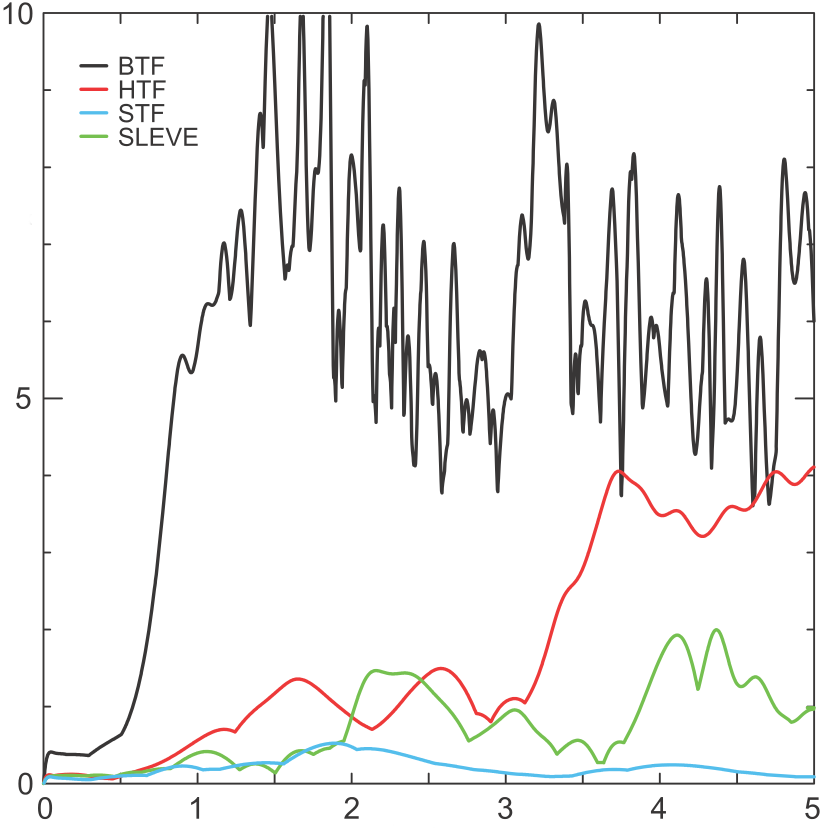
\includegraphics[height=2in]{img/klemp-w.png}}
	\caption{Maximum spurious vertical velocity $w$ in the resting atmosphere test compared with results from \textcite{klemp2011}.  Note that vertical scales differ.}
	\label{fig:resting:w}
\end{figure}

Test results for BTF, optimised SLEVE, and SnapCol grids are compared with results on a regular grid with no orography.  On the BTF grid, spurious vertical velocity $w$ reaches $\sim \SI{0.35}{\meter\per\second}$, which is significantly less than the velocities of $\sim \SI{10}{\meter\per\second}$ found by \textcite{klemp2011} (see figure~\ref{fig:resting:w}, note different vertical scales).  An oscillation develops after 4 hours, the cause of which is not yet known.  Unlike the results from \textcite{klemp2011}, the optimised SLEVE grid does not significantly reduce $w$ compared to BTF.  Since the model and its initialisation are the same, results on the BTF and optimised SLEVE grids are also in agreement with \textcite{weller-shahrokhi2014}.

The SnapCol grid results in a significantly smaller maximum vertical velocity of less than \SI{1e-3}{\meter\per\second}.  The smallest error of $\sim \SI{1e-10}{\meter\per\second}$ is found on the regular grid.  This error may be due to loss of precision when OpenFOAM loads the initial conditions, which are in discrete hydrostatic balance, but the source of the error is not certain.

\begin{figure}
	\captionsetup[subfigure]{position=b}
	\centering
	\subcaptionbox{Cell centres at centre of uncut cells leading to some cell centres below the ground \label{fig:resting:good:uncut}}[0.49\textwidth]{\input{resting-good-uncut-plot}}
	\hfill
	\subcaptionbox{Cell centres at centre of cut cells \label{fig:resting:good:cut}}[0.49\textwidth]{\input{resting-good-cut-plot}}
%
	\caption{Placement of cell centres on a two-dimensional cut cell grid.  The model from \textcite{good2013} has some cell centres below the ground (B. Good 2014, personal communication).  The arrows denote an estimated horizontal gradient between two adjacent cells of a scalar value stored at cell centres.}
	\label{fig:resting:good}
\end{figure}

Using a timestep of \SI{1.01}{\second}, \textcite{good2013} found the maximum vertical velocity in their cut cell model was \SI{1e-12}{\meter\per\second}, which is better than any result from the experiments in this project.  However, in that model, cell centres are in the centre of the uncut cell, resulting in the centre of some cut cells being below the ground, as shown in figure~\ref{fig:resting:good} (B. Good 2014, personal communication).  This means that the grid is effectively regular when calculating horizontal and vertical gradients.

\begin{figure}
	\captionsetup[subfigure]{position=b}
	\centering
	\subcaptionbox{Total normalised energy changes on terrain following grids \label{fig:resting:energy:total-tf}}[0.32\textwidth]{\input{resting-energy-total-tf-plot}}
	\hfill
	\subcaptionbox{As (\subcaptionref{fig:resting:energy:total-tf}), but on the SnapCol grid \label{fig:resting:energy:total-snapCol}}[0.32\textwidth]{\input{resting-energy-total-snapCol-plot}}
	\hfill
	\subcaptionbox{As (\subcaptionref{fig:resting:energy:total-tf}), but on a regular grid with no orography \label{fig:resting:energy:total-noOrography}}[0.32\textwidth]{\input{resting-energy-total-noOrography-plot}}
	\\
	\subcaptionbox{Kinetic ($E_K$), potential ($E_P$) and internal ($E_I$) normalised energy changes on BTF grid \label{fig:resting:energy:btf}}[0.32\textwidth]{\input{resting-energy-btf-plot}}
	\hfill
	\subcaptionbox{As (\subcaptionref{fig:resting:energy:btf}), but on the optimised SLEVE grid \label{fig:resting:energy:sleve}}[0.32\textwidth]{\input{resting-energy-sleve-plot}}
	\hfill
	\subcaptionbox{As (\subcaptionref{fig:resting:energy:btf}), but on the SnapCol grid.  Note the different vertical scale from figures~(\subcaptionref{fig:resting:energy:btf}) and (\subcaptionref{fig:resting:energy:sleve}). \label{fig:resting:energy:snapCol}}[0.32\textwidth]{\input{resting-energy-snapCol-plot}}
	\caption{Comparison of normalised energy changes on BTF, optimised SLEVE and SnapCol grids for the resting atmosphere test.}
	\label{fig:resting:energy}
\end{figure}

Examining normalised energy change, shown in figure~\ref{fig:resting:energy:total-tf}, we find that there is a net loss of energy on BTF and optimised SLEVE grids.  However, there is a period of energy gain on the optimised SLEVE grid during the first two hours, and an upward trend in energy after 3 hours on the BTF grid.  The cause of the energy gain is the subject of further work (see chapter~\ref{sec:further-work}).

Energy is better conserved on the SnapCol grid, the energy loss being more than two orders of magnitude smaller than the terrain following grids (figure~\ref{fig:resting:energy:total-snapCol}).  This compares favourably with the best possible energy conservation for this model as found on a regular grid (figure~\ref{fig:resting:energy:total-noOrography}).

The spurious motion generated by horizontal pressure gradient errors leads to a positive change in kinetic energy, evident in figures~\ref{fig:resting:energy:btf} and~\ref{fig:resting:energy:sleve}.  Compared to both terrain following grids, internal and potential energy conservation is three orders of magnitude better on the SnapCol grid (\ref{fig:resting:energy:snapCol}).  As noted by \textcite{weller-shahrokhi2014}, the model converts between potential and internal energy on timescales of less than an hour.  This can be seen by the mirroring between $E_P$ and $E_I$ plots, and we confirm that this local energy conservation property is present in all three grids (figures~\ref{fig:resting:energy:btf}, \subcaptionref{fig:resting:energy:sleve} and \subcaptionref{fig:resting:energy:snapCol}).

